\documentclass[12pt]{article}

\usepackage[spanish]{babel}
\usepackage[utf8]{inputenc}
\usepackage{graphicx}
\usepackage{geometry}
\usepackage{xcolor}
\usepackage{fancyhdr}
\usepackage{lastpage}
\usepackage{pdfpages}
\usepackage{listings}
\usepackage{schemata}

\geometry{top=25mm,left=15mm,right=15mm,a4paper}

\pagestyle{fancy}
\fancyhf{}
\lhead{Computación Concurrente}
\cfoot{Página \thepage\ de \pageref{LastPage}}

\graphicspath{./}

\begin{document}
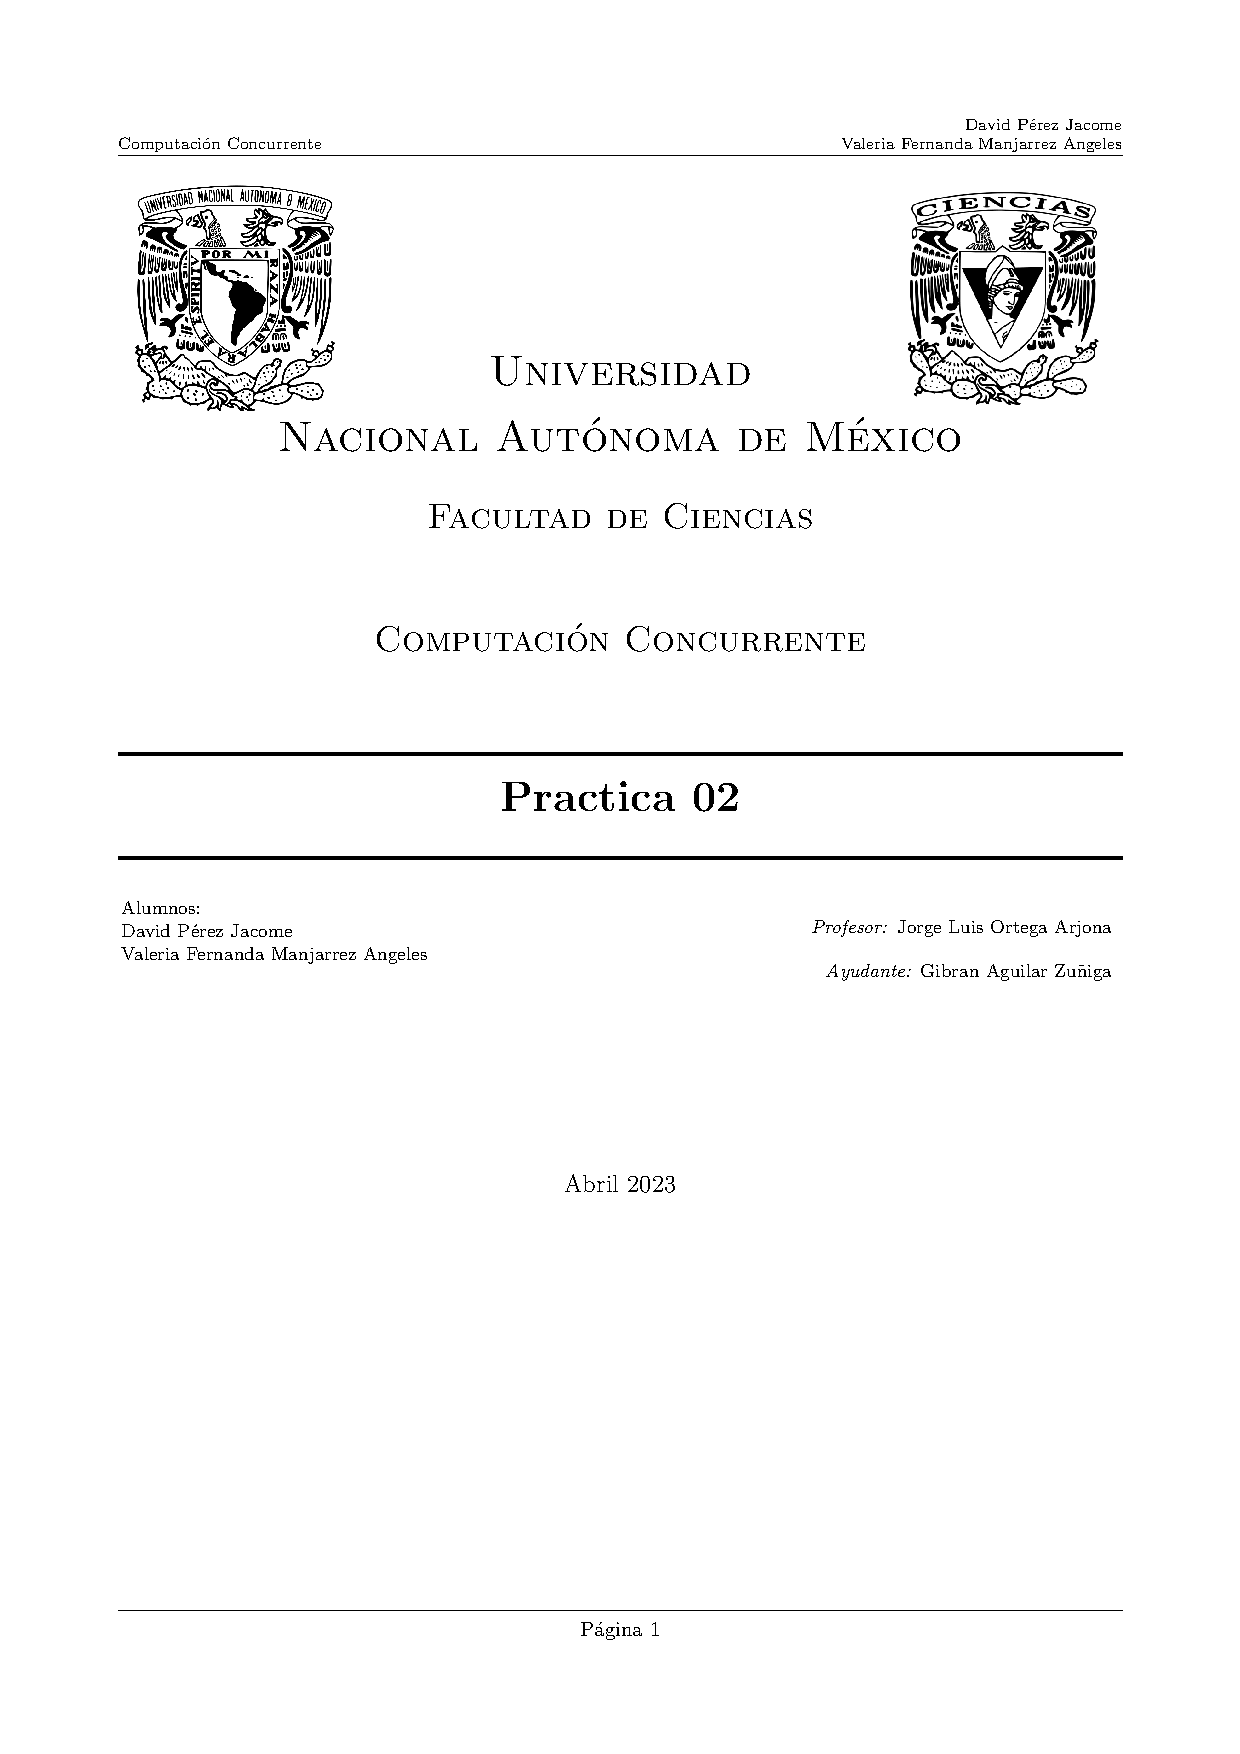
\includepdf{Portada.pdf}
{\color{red} \section*{\textbf{PRACTICA 02}}}
\vspace{1em}

{\color{blue} \subsection*{\textbf{Preguntas:}}}


Deberán detallar a profundidad las respuestas y en caso de ser necesario hacer diagramas 
para ejemplificar tu respuesta.\\


\begin{enumerate}
    \item ¿Qué es un proceso? (1 punto).
    \vspace{2mm}
    
    \textbf{Respuesta}
    \item ¿Qué es la sección crítica de un  proceso? (1 punto).
    \vspace{2mm}
    
    \textbf{Respuesta}
    \item ¿Qué es el problema libre de hambruna (2 puntos).
    \vspace{2mm}
    
    \textbf{Respuesta}
    \item ¿Qué es el problema de abrazos mortales? (2 puntos).
    \vspace{2mm}
    
    \textbf{Respuesta}
    \item Haz un TDA de Hilos y  un TDA de Semáforos (4 puntos).
    \vspace{2mm}
    
    \textbf{Respuesta}
\end{enumerate}







\end{document}